
\begin{figure}[ht!]
	\captionsetup{justification=justified, singlelinecheck=false, width=1\textwidth}
    \caption{Mapa do Brasil mostrando pontos de interesse e os epicentros dos eventos classificados como detonações e sismos. Foram detectados um total de sessenta e sete (67) eventos associados a detonações no período, classificados a partir do horário de ocorrência e da forma de onda, além do plano de fogo fornecido, com magnitudes mínima e máxima de 0.4 e 3.0 MLv, respectivamente.}
    \begin{mdframed}[
        linecolor=black,
        linewidth=1pt,
        roundcorner=10pt,
    ]
    \begin{center}
    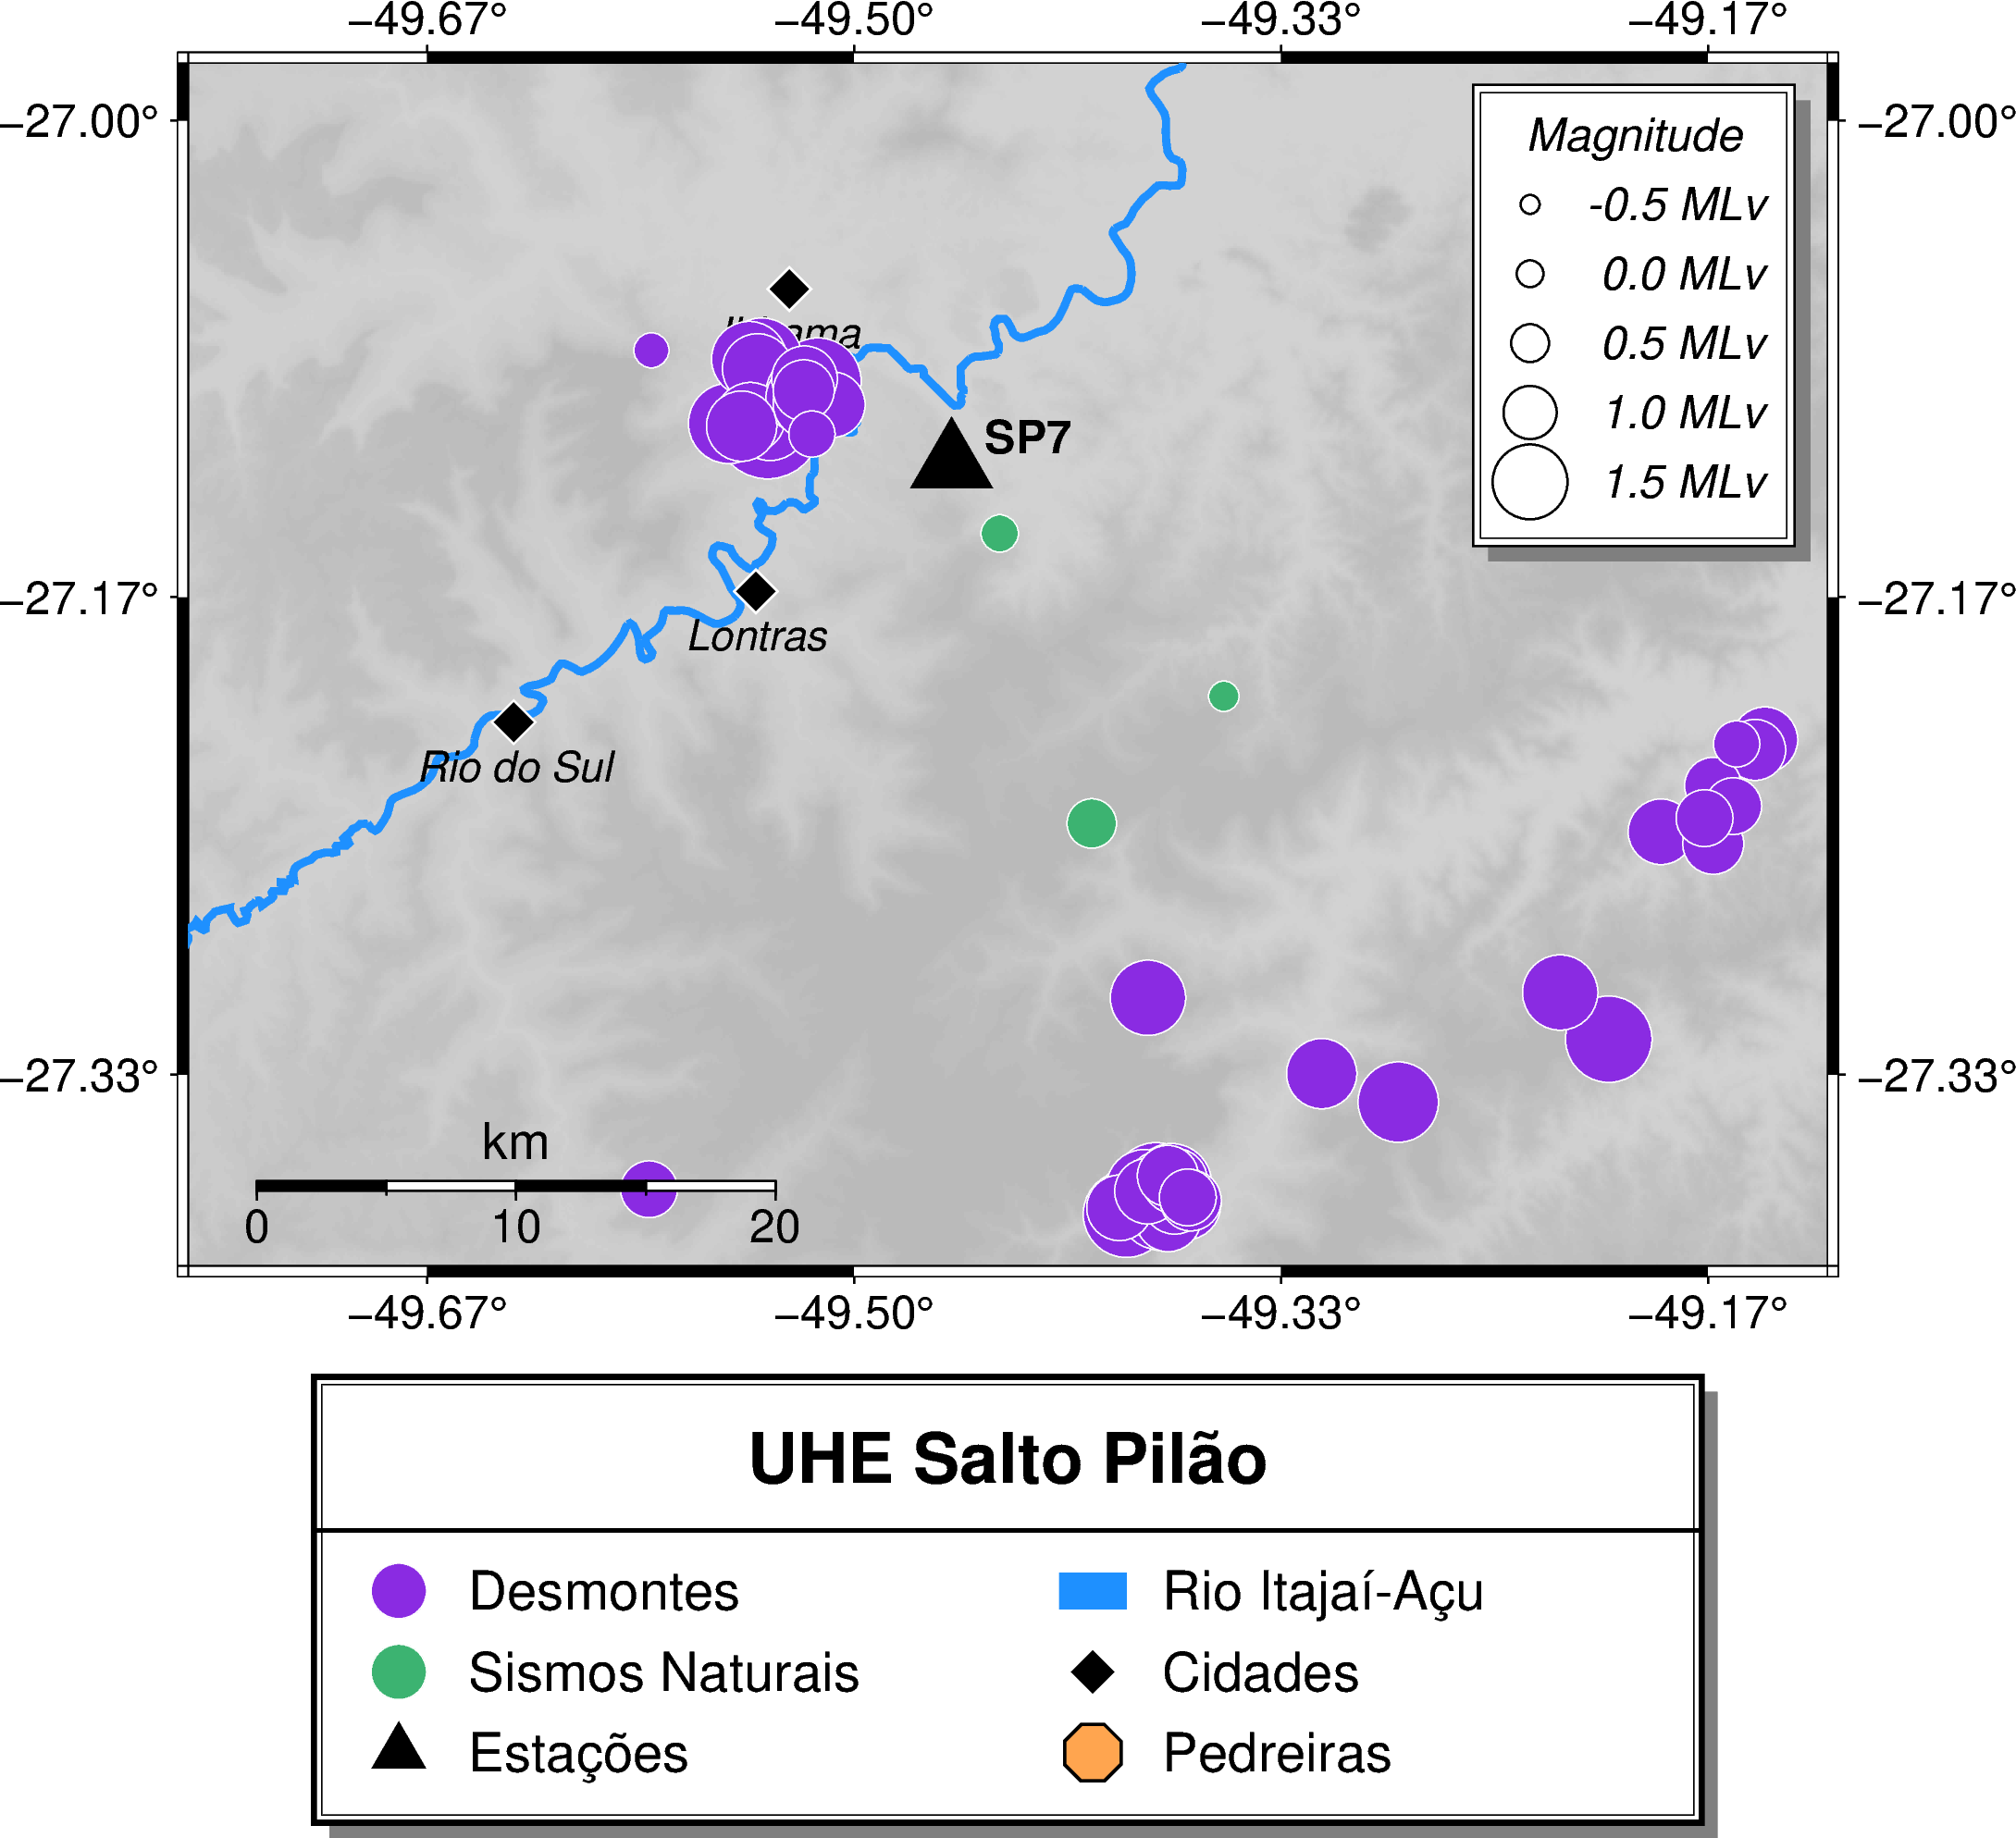
\includegraphics[width=0.8\textwidth]{/home/ggrl/projetos/ClassificadorSismologico/files/figures/maps/mapa.png}
    \end{center}
    \end{mdframed}
    \caption*{Fonte: IPT}
\end{figure}
